%------------------------------------------------------------------------------------------------------------------------------------------------------------------------------------------
% The Beamer class comes with a number of default slide themes
% which change the colors and layouts of slides. Below this is a list
%------------------------------------------------------------------------------------------------------------------------------------------------------------------------------------------
% of all the themes, uncomment each in turn to see what they look like.% As well as themes, the Beamer class has a number of color themes
% for any slide theme. Uncomment each of these in turn to see how it
% changes the colors of your current slide theme.
%------------------------------------------------------------------------------------------------------------------------------------------------------------------------------------------
%----------------------------------------------------------------------------------------
%	Packages
%----------------------------------------------------------------------------------------
\documentclass{beamer}
\usepackage{graphicx}
\usepackage{booktabs} % Allows the use of \toprule, \midrule and \bottomrule in tables
\usepackage{multicol}
\graphicspath{{Figures/}}
\mode<presentation> {
%----------------------------------------------------------------------------------------
%	Templates
%----------------------------------------------------------------------------------------
%\setbeamertemplate{footline} % To remove the footer line in all slides uncomment this line
\setbeamertemplate{footline}[page number] % To replace the footer line in all slides with a simple slide count uncomment this line
\setbeamertemplate{navigation symbols}{} % To remove the navigation symbols from the bottom of all slides uncomment this line
%----------------------------------------------------------------------------------------
%	Themes
%----------------------------------------------------------------------------------------
%\usetheme{default}
%\usetheme{AnnArbor}
%\usetheme{Antibes}
%\usetheme{Bergen}
%\usetheme{Berkeley}
%\usetheme{Berlin}
%\usetheme{Boadilla}
%\usetheme{CambridgeUS}
%\usetheme{Copenhagen}
%\usetheme{Darmstadt}
%\usetheme{Dresden}
%\usetheme{Frankfurt}
%\usetheme{Goettingen}
%\usetheme{Hannover}
%\usetheme{Ilmenau}
%\usetheme{JuanLesPins}
%\usetheme{Luebeck}
%\usetheme{Madrid}
%\usetheme{Malmoe}
\usetheme{Marburg}
%\usetheme{Montpellier}
%\usetheme{PaloAlto}
%\usetheme{Pittsburgh}
%\usetheme{Rochester}
%\usetheme{Singapore}
%\usetheme{Szeged}
%\usetheme{Warsaw}
%----------------------------------------------------------------------------------------
%	Color Themes
%----------------------------------------------------------------------------------------
%\usecolortheme{albatross}
%\usecolortheme{beaver}
%\usecolortheme{beetle}
%\usecolortheme{crane}
%\usecolortheme{dolphin}
%\usecolortheme{dove}
%\usecolortheme{fly}
\usecolortheme{lily}
%\usecolortheme{orchid}
%\usecolortheme{rose}
%\usecolortheme{seagull}
%\usecolortheme{seahorse}
%\usecolortheme{whale}
%\usecolortheme{wolverine}
}
%----------------------------------------------------------------------------------------
%	TITLE PAGE
%----------------------------------------------------------------------------------------
\title[Motion of Three Bodies in Space]{The Dynamics of a Triple Celestial Body System} % The short title appears at the bottom of every slide, the full title is only on the title page
\author{Taylor Larrechea} % Your name
\institute[CMU] % Your institution as it will appear on the bottom of every slide, may be shorthand to save space
{
Colorado Mesa University \\ % Your institution for the title page
\medskip
}
\date{October 31, 2019} % Date, can be changed to a custom date
%----------------------------------------------------------------------------------------
%	Begin Document
%----------------------------------------------------------------------------------------
\begin{document}
\begin{frame}
\titlepage % Print the title page as the first slide
\end{frame}
%----------------------------------------------------------------------------------------
%	Presentation Slides
%----------------------------------------------------------------------------------------
%------------------------------------------------
%	Table of Contents
%------------------------------------------------
\begin{frame}
\frametitle{Table of Contents} % Table of contents slide, comment this block out to remove it
\tableofcontents % Throughout your presentation, if you choose to use \section{} and \subsection{} commands, these will automatically be printed on this slide as an overview of your presentation
\end{frame}
%------------------------------------------------
%	Main Purpose of Project
%------------------------------------------------
\section{Main Purpose of Project}
\begin{frame}
\frametitle{Main Purpose of Project}
To plot the motion of three massive bodies in space orbiting one another using computational methods and Newtonian Gravitation.
\begin{figure}[htpb]
\begin{center}
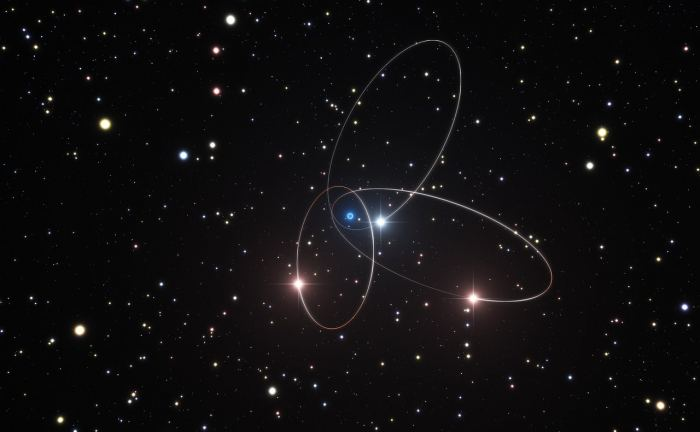
\includegraphics[width=0.85\linewidth]{Stars.jpg} 
\end{center}
\end{figure}
Find initial conditions that would be optimal to use in the search of ternary star systems.
\end{frame}
%------------------------------------------------
%	Multiple Star Systems
%------------------------------------------------
\subsection{\tiny{Multiple Star Systems}}
\begin{frame}
\frametitle{Multiple Star System}
Most star systems are binary at the least. In fact, 85\% of star systems are binary at least \cite{CSIRO}.
\begin{figure}
\begin{center}
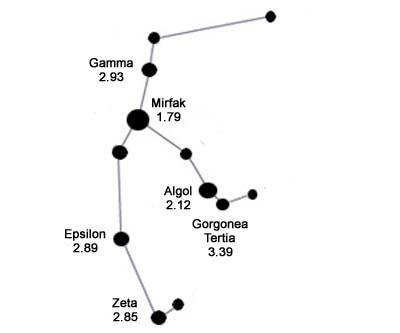
\includegraphics[width=0.70\linewidth]{Perseus.jpg}
\end{center}
\end{figure}
\end{frame}
%------------------------------------------------
%	Methodology of Plotting Motion
%------------------------------------------------
\section{Methodology of Plotting Motion}
\begin{frame}
\frametitle{Methodology of Plotting Motion}
We must first identify the differential equations that we plan to solve in order to plot the motion of our massive bodies in space  \\
\begin{equation*}
F(\vec{r})=m\frac{d^2\vec{r}}{dt^2}
\end{equation*}\\
where $F(\vec{r})$ is
\begin{equation}\label{1}
\vec{F}=\frac{GMm}{r^2}(\hat{n}).
\end{equation}
Numerical methods are needed to solve these difficult differential equations.
\end{frame}
%------------------------------------------------
%	F.E.D.S (1)
%------------------------------------------------
\subsection{\tiny{F.E.D.S - Forward Euler Difference Scheme}}
\begin{frame}
\frametitle{Forward Euler Difference Scheme (1)}
The differential equations that describe the acceleration of three bodies in space will have to be solved via numerical techniques with Python.\\
\vspace{20pt}
A typical method that is used to solve differential equations numerically is a Forward Euler Difference Scheme, or F.E.D.S for short \cite{Forward Euler Difference Scheme}
\begin{equation}\label{2}
y_{n+1}=y_{n}+h\hspace{1pt}f(x_{n},y_{n}).
\end{equation}
A time step of 0.0001 seconds was used in this algorithm.
\end{frame}
%------------------------------------------------
%	F.E.D.S (2)
%------------------------------------------------
\begin{frame}
\frametitle{Forward Euler Difference Scheme (2)}
Typically, the F.E.D.S is the simplest Runge-Kutta scheme there is for solving first order differential equations.
\begin{figure}[htbp]
\begin{center}
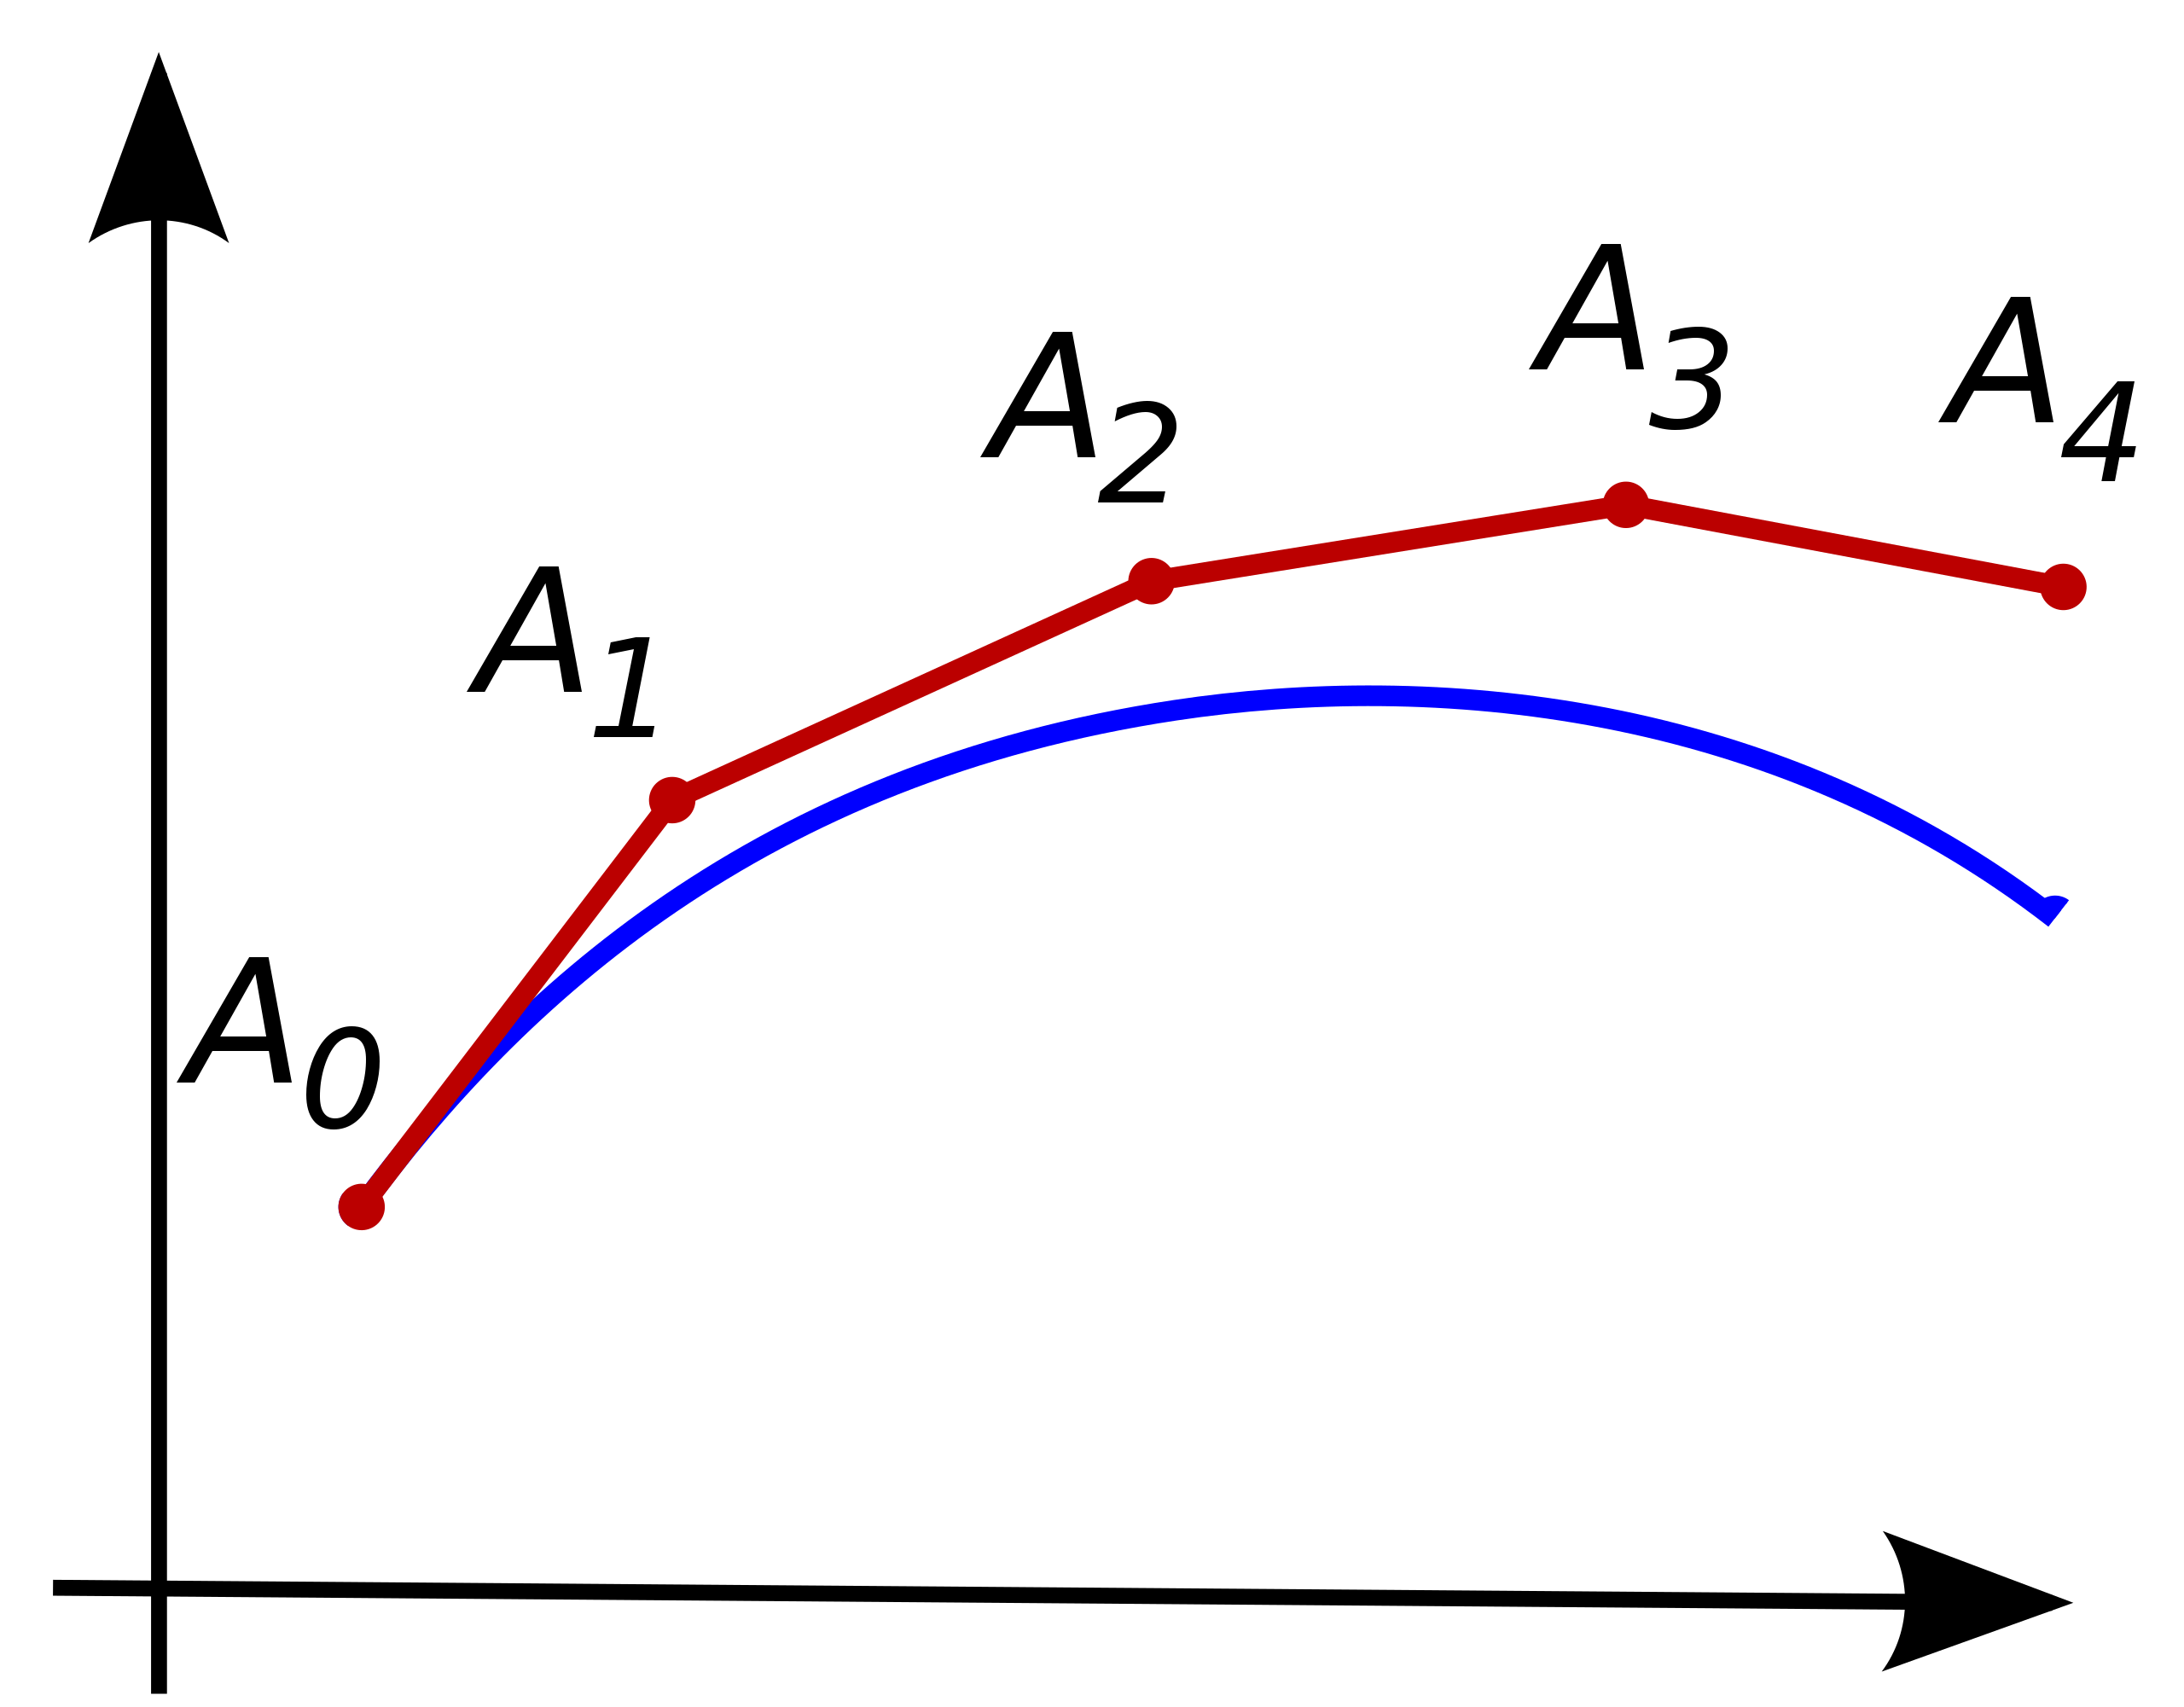
\includegraphics[width=0.50\linewidth]{EulerMethod.png}
\end{center}
\end{figure}
\end{frame}
%------------------------------------------------
%	F.E.D.S (3)
%------------------------------------------------
\begin{frame}
\frametitle{Forward Euler Difference Scheme (3)}
To have an understanding of how our equations of emotion develop, examine the following image.
\begin{figure}[htbp]
\begin{center}
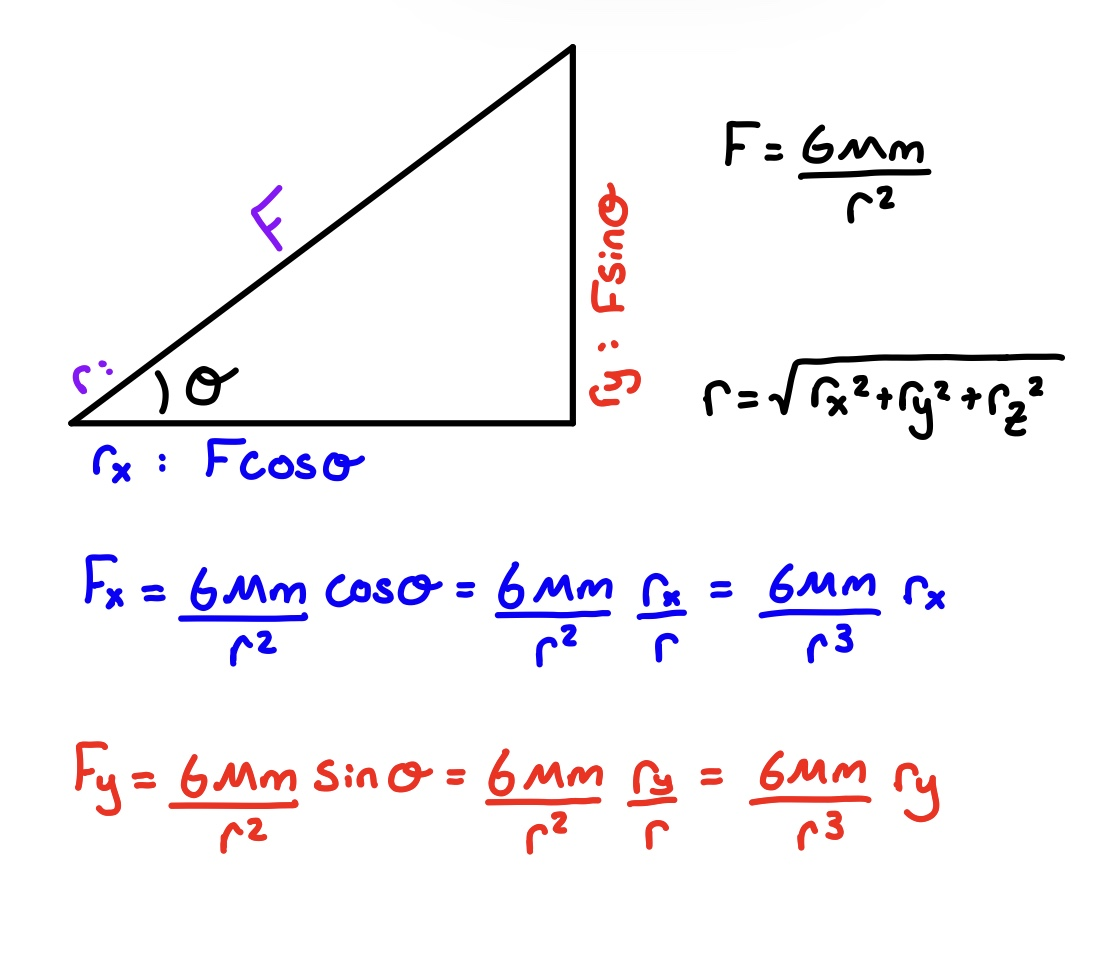
\includegraphics[width=0.75\linewidth]{ForceDiagram.png}
\end{center}
\end{figure}
\end{frame}
%------------------------------------------------
%	F.E.D.S (4) 
%------------------------------------------------
\begin{frame}
\frametitle{Forward Euler Difference Scheme (4)}
For simplicity's sake, we will only examine the two body equations.
\\
\vspace{10pt}
Beginning with the distance between bodies
\begin{equation*}
r_x=x_{2}-x_{1},
\end{equation*}
\begin{equation*}
r_y=y_{2}-y_{1}, 
\end{equation*}
\begin{equation*}
r_z=z_{2}-z_{1},
\end{equation*}
\begin{equation*}
r=\sqrt{r_x^2+r_y^2+r_z^2}
\end{equation*}
we now have a way to quantify the distance between the two bodies in space.
\end{frame}
%------------------------------------------------
%	F.E.D.S (5)
%------------------------------------------------
\begin{frame}
\frametitle{Forward Euler Difference Scheme (5)}
Now the force between the bodies of mass can be calculated
\begin{equation*}
f_x=-\frac{Gm_{1}m_{2}}{(r_{x}^2+r_{y}^2+r_{z}^2)^{3/2}}(r_x),
\end{equation*}
\begin{equation*}
f_y=-\frac{Gm_{1}m_{2}}{(r_{x}^2+r_{y}^2+r_{z}^2)^{3/2}}(r_y),
\end{equation*}
\begin{equation*}
f_z=-\frac{Gm_{1}m_{2}}{(r_{x}^2+r_{y}^2+r_{z}^2)^{3/2}}(r_z)
\end{equation*}
giving us three equations that we can use to find the force between our bodies of mass.
\end{frame}
%------------------------------------------------
%	F.E.D.S (6)
%------------------------------------------------
\begin{frame}
\frametitle{Forward Euler Difference Scheme (6)}
Next with updating the velocities for mass one
\begin{equation*}
v_{x_{1}}+=-\frac{f_x}{m_1}\cdot dt,
\end{equation*}
\begin{equation*}
v_{y_{1}}+=-\frac{f_y}{m_1}\cdot dt,
\end{equation*}
\begin{equation*}
v_{z_{1}}+=-\frac{f_z}{m_1}\cdot dt,
\end{equation*}
we can now update the velocities in each direction of one body. 
\end{frame}
%------------------------------------------------
%	F.E.D.S (7)
%------------------------------------------------
\begin{frame}
\frametitle{Forward Euler Difference Scheme (7)}
We now can begin to update the positions of our bodies of mass. Updating the positions for mass one
\begin{align*}
x_{1}&+=v_{x_{1}}\cdot dt, \\
y_{1}&+=v_{y_{1}}\cdot dt, \\
z_{1}&+=v_{z_{1}}\cdot dt, \\
t&+=dt,
\end{align*}
we are now in position to plot these positions.
\end{frame}
%------------------------------------------------
%	F.E.D.S (8)
%------------------------------------------------
\begin{frame}
\frametitle{Forward Euler Difference Scheme (8)}
Let's examine the distance on mass 1 due to mass 2 and mass 3. The distances between the masses are
\begin{equation*}
r_{12}=(r_{12x}^2+r_{12y}^2+r_{12z}^2)^{3/2},
\end{equation*}
\begin{equation*}
r_{13}=(r_{13x}^2+r_{13y}^2+r_{13z}^2)^{3/2}.
\end{equation*}
With the above equations we can now calculate the force between the three bodies.
\end{frame}
%------------------------------------------------
%	F.E.D.S (9)
%------------------------------------------------
\begin{frame}
\frametitle{Forward Euler Difference Scheme (9)}
The forces in each direction can now be calculated. The equations that were fed into python are
\begin{equation*}
f_{x}=-\frac{Gm_1m_2}{r_{12}}(r_{{12}_x})-\frac{Gm_1m_3}{r_{13}}(r_{13x}),
\end{equation*}
\begin{equation*}
f_{y}=-\frac{Gm_1m_2}{r_{12}}(r_{{12}_y})-\frac{Gm_1m_3}{r_{13}}(r_{13y}),
\end{equation*}
\begin{equation*}
f_{z}=-\frac{Gm_1m_2}{r_{12}}(r_{{12}_z})-\frac{Gm_1m_3}{r_{13}}(r_{13z}),
\end{equation*}
which now can be used to calculate new velocities and positions.
\end{frame}
%------------------------------------------------
%	F.E.D.S (10)
%------------------------------------------------
\begin{frame}
\frametitle{Forward Euler Difference Scheme (10)}
The only difference between the two body and three body system is how the distance between the bodies are calculated and the forces between the bodies are calculated.
\begin{figure}[htpb]
\begin{center}
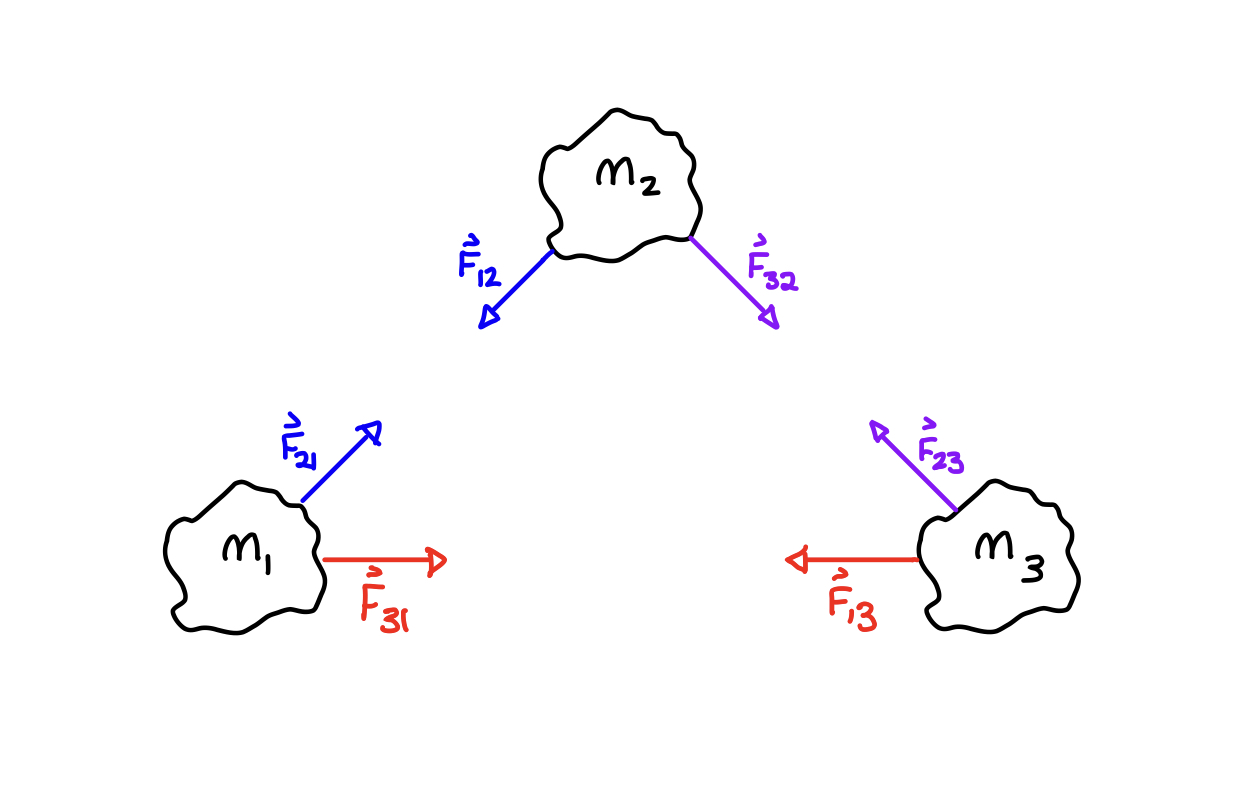
\includegraphics[width=0.85\linewidth]{3BodyCartoon1.png} 
\end{center}
\end{figure}
\end{frame}
%------------------------------------------------
%	F.E.D.S (11)
%------------------------------------------------
\begin{frame}
\frametitle{Forward Euler Difference Scheme (11)}
Now that the groundwork is laid for how to solve the equations of motion, we can begin to start on the actual work that involves solving these differential equations.
\begin{figure}[htpb]
\begin{center}
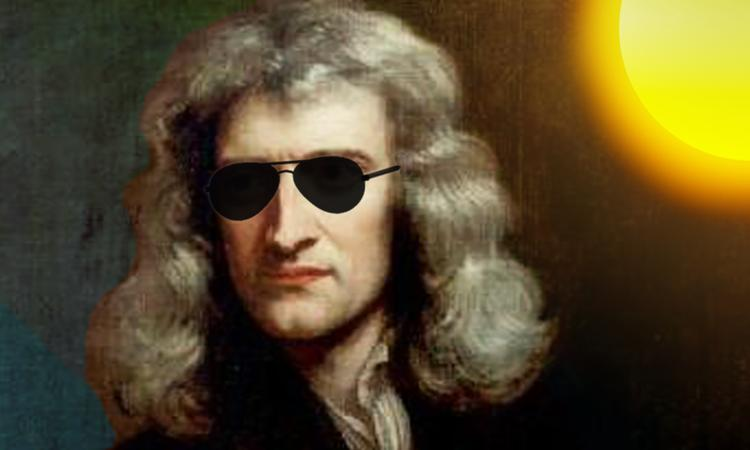
\includegraphics[width=0.85\linewidth]{IsaacNewton.jpg} 
\end{center}
\end{figure}
\end{frame}
%------------------------------------------------
%	Simple 1-D Motion (1)
%------------------------------------------------
\section{Simple 1-D Motion}
\begin{frame}
\frametitle{Simple 1-D Motion (1)}
The simplest scenario for this project is 1-D motion. First we will solve for the motion of a ball being thrown in the air so high that we cannot just assume $\vec{a}=g$, assuming that it only has vertical motion.
\begin{figure}[htbp]
\begin{center}
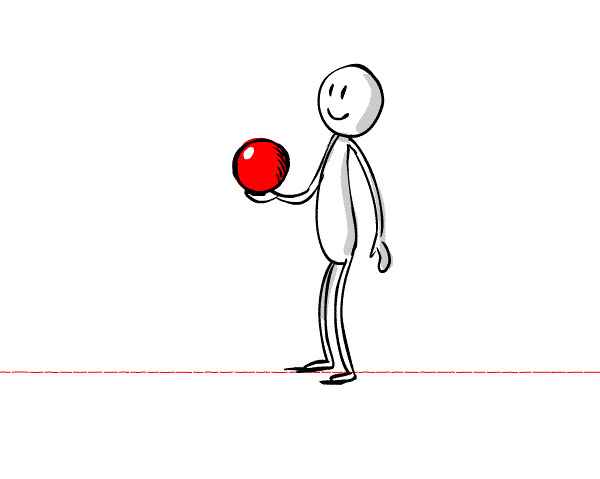
\includegraphics[width=0.50\linewidth]{Cartoon1.jpg}
\end{center}
\end{figure}
\end{frame}
%------------------------------------------------
%	Simple 1-D Motion (2)
%------------------------------------------------
\begin{frame}
\frametitle{Simple 1-D Motion (2)}
We will first start with Newtonian Gravity
\begin{equation}\label{3}
\vec{F}=\frac{GMm}{r^2}
\end{equation}
where \textit{r} is the distance from the center of a body of mass. Using the formula for Force where mass is constant we have
\begin{equation}\label{4}
\vec{F}=m\vec{a}.
\end{equation}
Rearranging equations (3) and (4) we have our equation for acceleration
\begin{equation}\label{5}
\vec{a}=\frac{GM}{r^2}.
\end{equation}
\end{frame}
%------------------------------------------------
%	Simple 1-D Motion (3)
%------------------------------------------------
\begin{frame}
\frametitle{Simple 1-D Motion (3)}
Our first goal with modeling 1-D motion is to get our code running so we can then progress to more complicated scenarios. Modifying equation (5) we can solve an equation for simple 1-D motion
\begin{equation}\label{6}
\vec{a}=\frac{GM}{r^2}
\end{equation}
where $R$ is the radius and $M$ is the mass the of Earth and $r=R+y$. The variable $y$ is an arbitrary value that we choose off of initial conditions.
\end{frame}
%------------------------------------------------
%	Simple 1-D Motion (4)
%------------------------------------------------
\begin{frame}
\frametitle{Simple 1-D Motion (4)}
Using equation (6) where the initial conditions of our ball being thrown is $v_{iy}=25$ $m/s$ and $y_{i}=100$ $m$, we get the following plot when the motion is solved for.
\begin{figure}[htbp]
\begin{center}
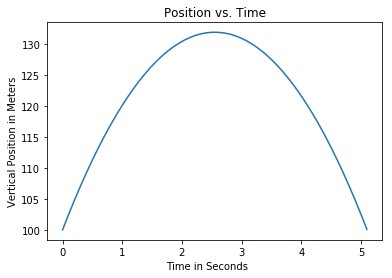
\includegraphics[width=0.75\linewidth]{1DMotion1.jpg}
\end{center}
\end{figure}
\end{frame}
%------------------------------------------------
%	Simple 1-D Motion (5)
%------------------------------------------------
\begin{frame}
\frametitle{Simple 1-D Motion (5)}
Neglecting air resistance we can find the time that it takes for our ball to reach the ground;
\begin{equation}\label{7}
V_{1}=V_{0}+a\triangle t, \hspace{5pt} V_{1}^2=V_{0}^2+2a\triangle x, \hspace{5pt} \triangle x = V_{0}\triangle t + \frac{1}{2}a\triangle t^2.
\end{equation}
Using these three equations the time that it takes for the ball to reach the ground is $\triangle t = 7.74 \hspace{2pt} (s)$.
\begin{figure}[htbp]
\begin{center}
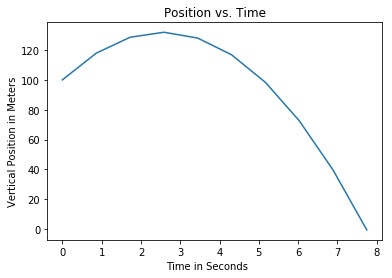
\includegraphics[width=0.70\linewidth]{1DMotion2.jpg}
\end{center}
\end{figure}
\end{frame}
%------------------------------------------------
%	Simple 1-D Motion (6)
%------------------------------------------------
\begin{frame}
\frametitle{Simple 1-D Motion (6)}
ODEint was used to solve the previous equations and plot their motion.\\
\vspace{20pt}
The next progression in this project was to plot 2-D kinematic motion, but because of time this part of the project was annexed and we moved on to 2-Body Motion.\\
\vspace{20pt}
Also, ODEint was not able to be used for a 2-D kinematic example and thus arose the necessity of developing my own code.
\end{frame}
%------------------------------------------------
%	2-Body Motion (1)
%------------------------------------------------
\section{2-Body Motion}
\begin{frame}
\frametitle{2-Body Motion (1)}
The purpose of modeling 1-D kinematic motion was to start with the easiest scenario and then progressively move towards more complicated scenarios.
\begin{figure}[htbp]
\begin{center}
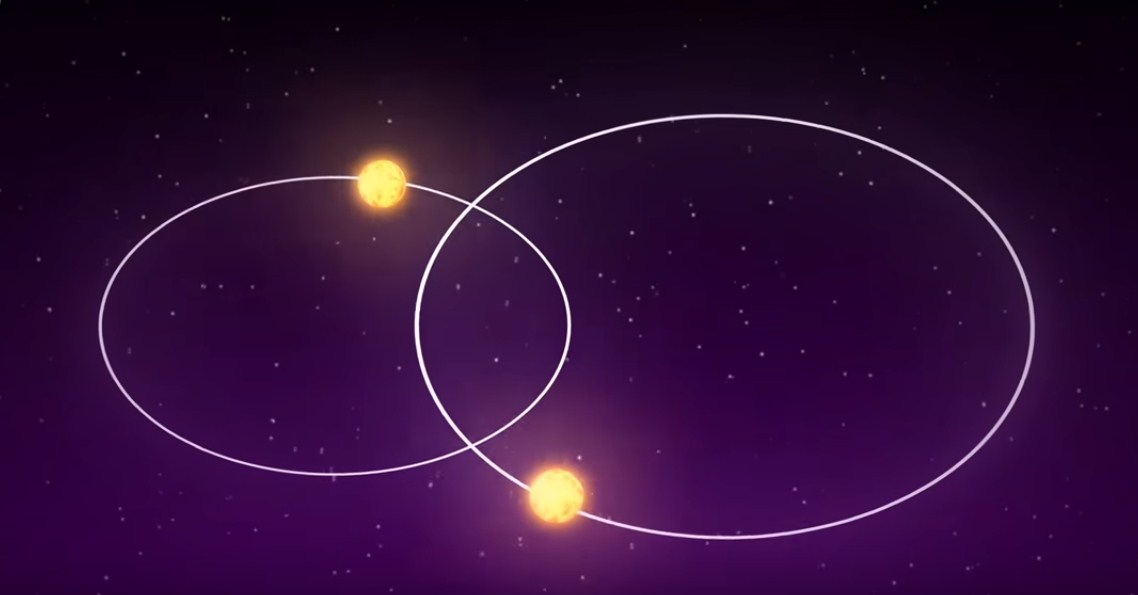
\includegraphics[width=0.70\linewidth]{BinaryStar.jpg}
\end{center}
\end{figure}
The next more complicated scenario is the motion of two bodies in space.
\end{frame}
%------------------------------------------------
%	2-Body Motion (2)
%------------------------------------------------
\begin{frame}
\frametitle{2-Body Motion (2)}
So let's begin with the simplest two body scenario, two bodies at rest.
\begin{figure}[htbp]
\begin{center}
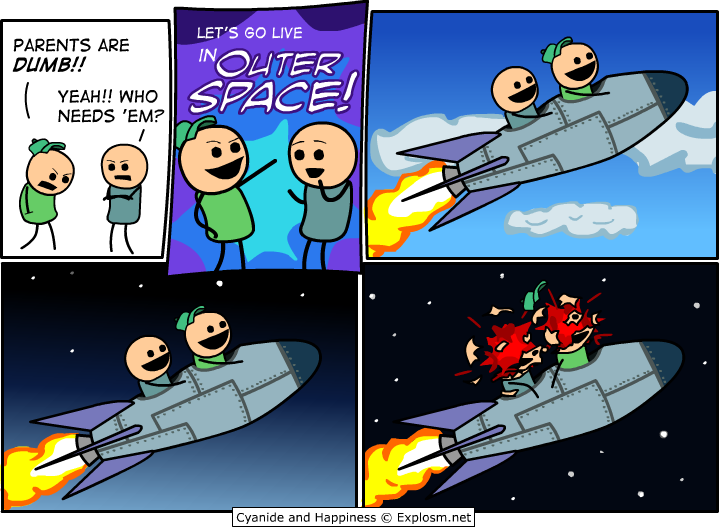
\includegraphics[width=0.75\linewidth]{SpaceComic.png}
\end{center}
\end{figure}
\end{frame}
%------------------------------------------------
%	2-Body Motion (3)
%------------------------------------------------
\begin{frame}
\frametitle{2-Body Motion (3)}
Here is an example of the 2-Body Code.
\begin{multicols}{2}
\begin{figure}
\begin{center}
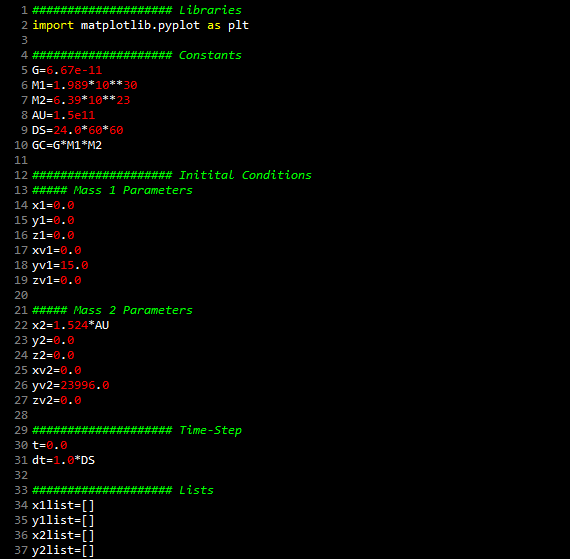
\includegraphics[width=1.0\linewidth]{2BodyCode1.png}
\end{center}
\end{figure}
\begin{figure}
\begin{center}
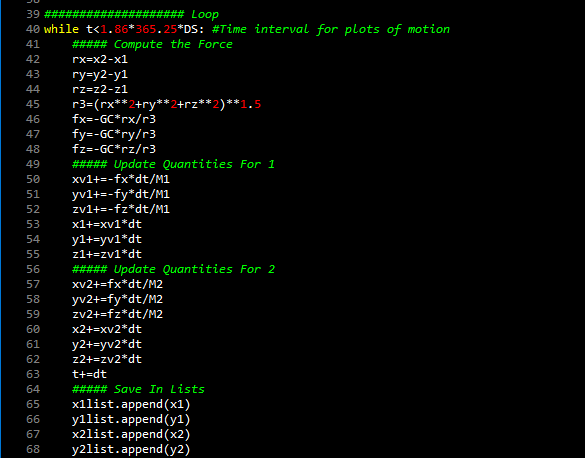
\includegraphics[width=1.0\linewidth]{2BodyCode2.png}
\end{center}
\end{figure}
\end{multicols}
\end{frame}
%------------------------------------------------
%	2-Body Motion (4)
%------------------------------------------------
\subsection{\tiny{Initial Force Attraction}}
\begin{frame}
\frametitle{2-Body Motion (4)}
Let's imagine two bodies of mass, $m_1=50 \hspace{2pt} kg$ and $m_2=100 \hspace{2pt} kg$ 200 meters apart originally.
\begin{figure}[htbp]
\begin{center}
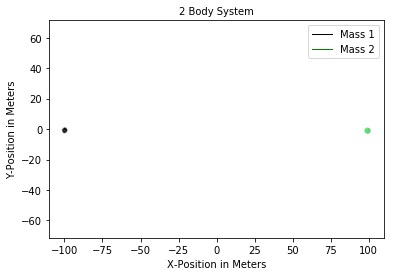
\includegraphics[width=0.85\linewidth]{2Body1.png}
\end{center}
\end{figure}
\end{frame}
%------------------------------------------------
%	2-Body Motion (5)
%------------------------------------------------
\begin{frame}
\frametitle{2-Body Motion (5)}
Intuitively, the bodies of mass should attract one another and eventually collide at a certain point. This journey takes $\approx$ 364 (Earth) days.
\begin{figure}[htbp]
\begin{center}
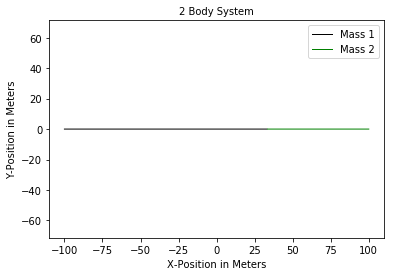
\includegraphics[width=0.70\linewidth]{2Body2.png}
\end{center}
\end{figure}
This confirms our code is working and we can move on to more complicated examples of 2 body motion.
\end{frame}
%------------------------------------------------
%	2-Body Motion (6)
%------------------------------------------------
\subsection{\tiny{Planetary Motion}}
\begin{frame}
\frametitle{2-Body Motion (6)}
Now that our code is working on the simplest of scales, we can begin to plot orbits that are commonly known.
\begin{figure}[htpb]
\begin{center}
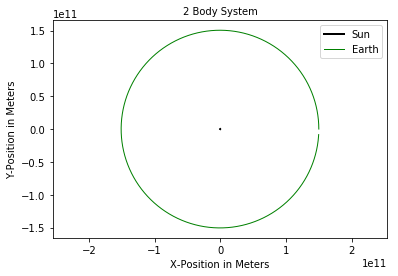
\includegraphics[width=0.75\linewidth]{Figures/EarthPlot.png} 
\end{center}
\end{figure}
The code actually took $\approx$ 368 days to complete one orbit giving a 1\% error in the code.
\end{frame}
%------------------------------------------------
%	2-Body Motion (7)
%------------------------------------------------
\begin{frame}
\frametitle{2-Body Motion (7)}
And one more plot that is commonly known.
\begin{figure}[htpb]
\begin{center}
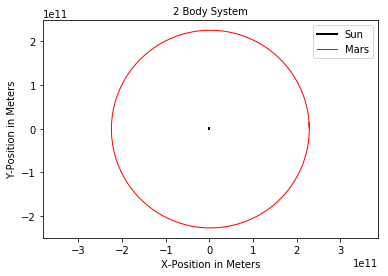
\includegraphics[width=0.75\linewidth]{Figures/MarsPlot.png} 
\end{center}
\end{figure}
In this plot, it only took $\approx$ 672 days to complete one orbit yielding $\approx$ a 2\% error.
\end{frame}
%------------------------------------------------
%	3-Body Motion (1)
%------------------------------------------------
\section{3-Body Motion}
\subsection{\tiny{Common Facts}}
\begin{frame}
\frametitle{3-Body Motion (1)}
The three body system is a very chaotic system, meaning the orbits are heavily dependent upon initial conditions. \\
\vspace{40pt}
The purpose of this part of the project was to probe initial conditions to determine what are suitable initial conditions for ternary systems.
\end{frame}
%------------------------------------------------
%	3-Body Motion (2)
%------------------------------------------------
\subsection{\tiny{Plots of 3-Body Motion}}
\begin{frame}
\frametitle{3-Body Motion (2)}
The first scenario that will be examined can be seen in the cartoon below.
\begin{figure}[htpb]
\begin{center}
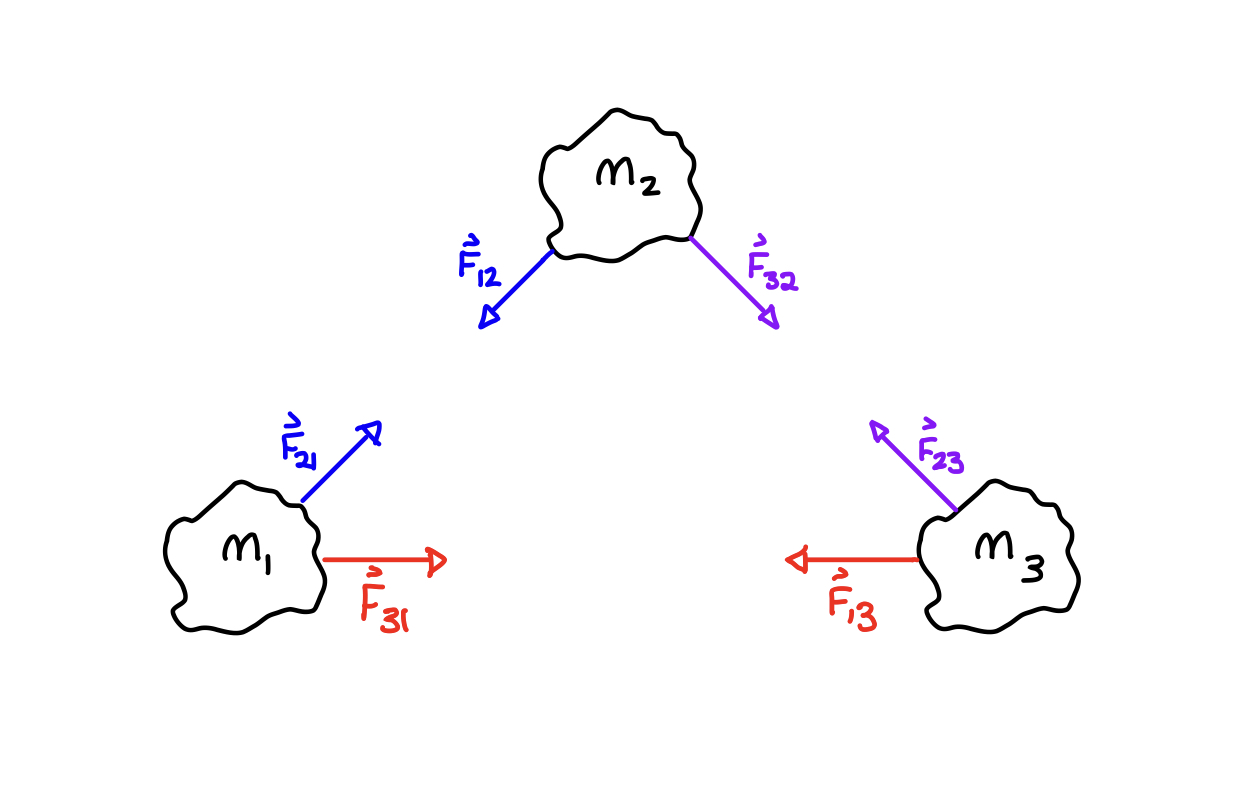
\includegraphics[width=0.85\linewidth]{3BodyCartoon1.png} 
\end{center}
\end{figure}
\end{frame}
%------------------------------------------------
%	3-Body Motion (3)
%------------------------------------------------
\begin{frame}
\frametitle{3-Body Motion (3)}
We will begin by examining a scenario of 3-bodies in space that are originally in an equilateral triangle orientation.
\begin{multicols}{2}
\begin{figure}
\begin{center}
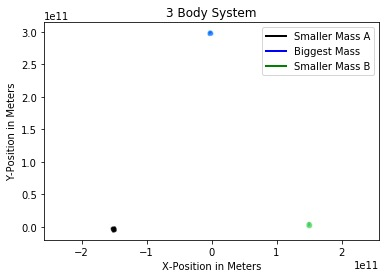
\includegraphics[width=1.0\linewidth]{3BodyDynamics1.png}
\end{center}
\end{figure}
\begin{figure}
\begin{center}
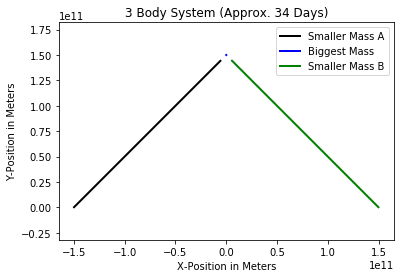
\includegraphics[width=1.0\linewidth]{3BodyDynamics2.png}
\end{center}
\end{figure}
\end{multicols}
The black and green masses are roughly equivalent to the mass of Earth. The blue mass is roughly that of our sun.
\end{frame}
%------------------------------------------------
%	3-Body Motion (4)
%------------------------------------------------
\begin{frame}
\frametitle{3-Body Motion (4)}
Now we begin plotting these bodies in motion. $M_1$ will be moving at $\approx 30,000$ m/s in the x-direction and $M_3$ will be moving at $\approx 30,000$ m/s in the y-direction.
\begin{multicols}{2}
\begin{figure}
\begin{center}
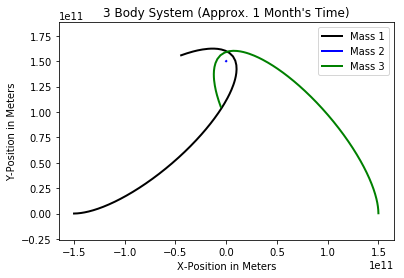
\includegraphics[width=1.0\linewidth]{3BodyDynamics3.png}
\end{center}
\end{figure}
\begin{figure}
\begin{center}
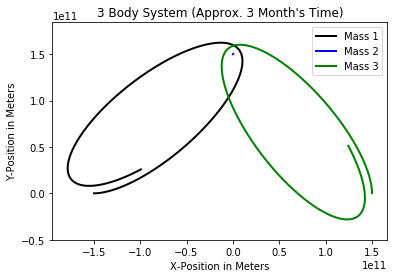
\includegraphics[width=1.0\linewidth]{3BodyDynamics4.png}
\end{center}
\end{figure}
\end{multicols}
\end{frame}
%------------------------------------------------
%	3-Body Motion (5)
%------------------------------------------------
\begin{frame}
\frametitle{3-Body Motion (5)}
Letting this system progress over time, we get the following plot after about three years.
\begin{figure}
\begin{center}
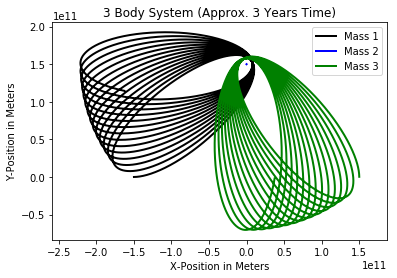
\includegraphics[width=0.90\linewidth]{3BodyDynamics5.png}
\end{center}
\end{figure}
\end{frame}
%------------------------------------------------
%	3-Body Motion (6)
%------------------------------------------------
\begin{frame}
\frametitle{3-Body Motion (6)}
Using the same initial starting conditions as the last plots, with $M_1=M_3=6\cdot10^{26}$ kg and both in motion at $\approx30,000$ m/s and $M_2$ at $\approx -30,000$ m/s the following plots are created.
\begin{multicols}{2}
\begin{figure}
\begin{center}
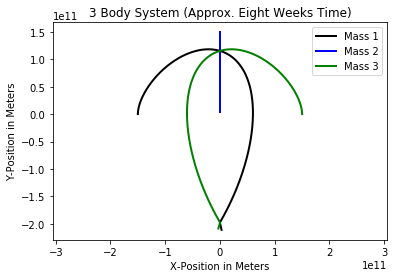
\includegraphics[width=1.0\linewidth]{3BodyDynamics13.png}
\end{center}
\end{figure}
\begin{figure}
\begin{center}
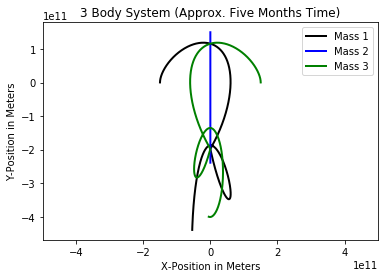
\includegraphics[width=1.0\linewidth]{3BodyDynamics14.png}
\end{center}
\end{figure}
\end{multicols}
\end{frame}
%------------------------------------------------
%	3-Body Motion (7)
%------------------------------------------------
\begin{frame}
\frametitle{3-Body Motion (7)}
Letting this system progress, the following final plot is created.
\begin{figure}
\begin{center}
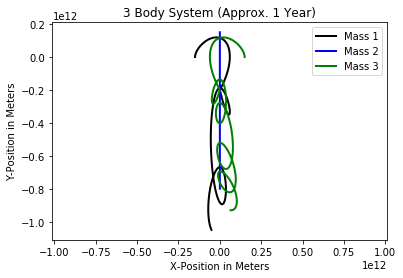
\includegraphics[width=0.90\linewidth]{3BodyDynamics15.png}
\end{center}
\end{figure}
\end{frame}
%------------------------------------------------
%	3-Body Motion (8)
%------------------------------------------------
\begin{frame}
\frametitle{3-Body Motion (8)}
We now examine a new scenario where the three bodies are all aligned in a horizontal manner.
\begin{figure}
\begin{center}
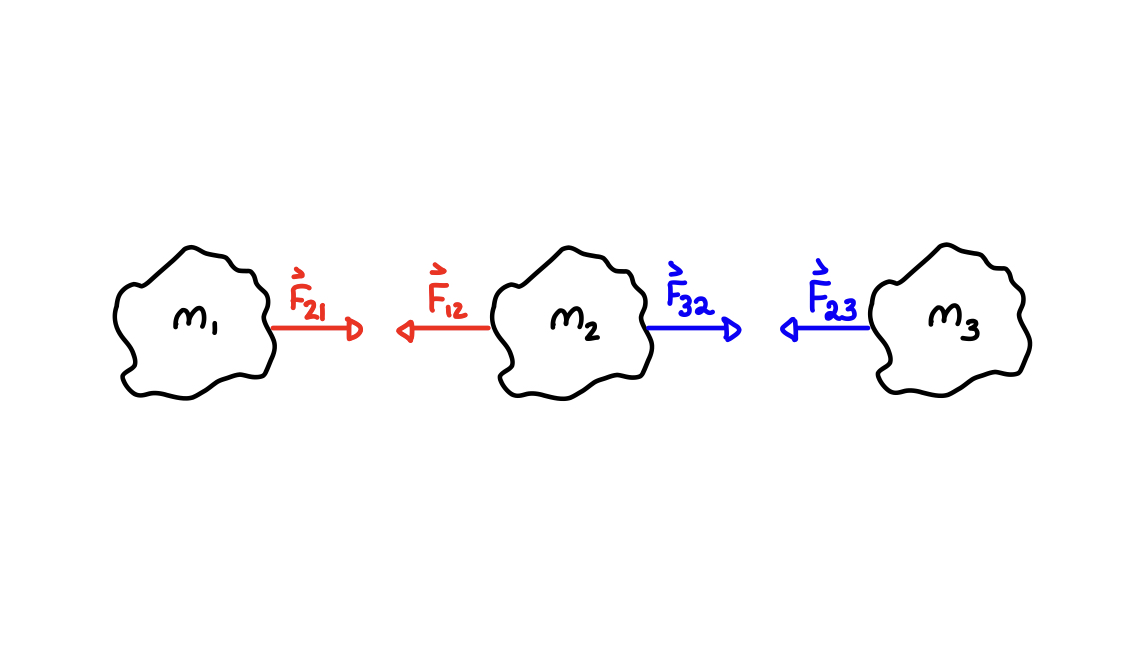
\includegraphics[width=0.80\linewidth]{3BodyCartoon3.png}
\end{center}
\end{figure}
The masses of $M_{1}$ and $M_{3}$ are $\approx 6.0\times 10^{29}$ kg.
\end{frame}
%------------------------------------------------
%	3-Body Motion (9)
%------------------------------------------------
\begin{frame}
\frametitle{3-Body Motion (9)}
Mass 1 and Mass 3 are both initially moving at a velocity of $v=50,000$ m/s, where Mass 1 is initially moving in the positive y-direction and Mass 3 is initially moving in the negative y-direction.
\begin{multicols}{2}
\begin{figure}
\begin{center}
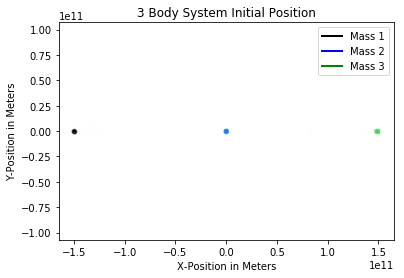
\includegraphics[width=1.0\linewidth]{3BodyDynamics6.png}
\end{center}
\end{figure}
\begin{figure}
\begin{center}
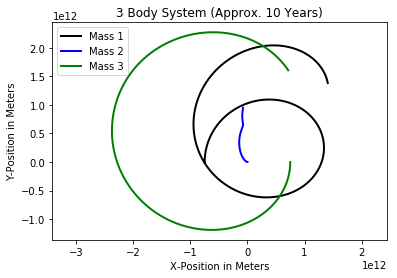
\includegraphics[width=1.0\linewidth]{3BodyDynamics7.png}
\end{center}
\end{figure}
\end{multicols}
\end{frame}
%------------------------------------------------
%	3-Body Motion (10)
%------------------------------------------------
\begin{frame}
\frametitle{3-Body Motion (10)}
This system evolves over time and the following plot is generated after about 20 years time.
\begin{figure}
\begin{center}
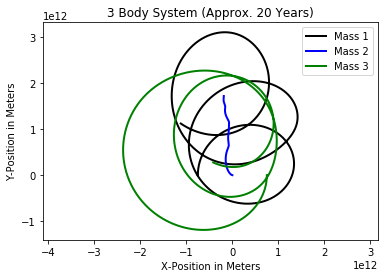
\includegraphics[width=0.90\linewidth]{3BodyDynamics8.png}
\end{center}
\end{figure}
\end{frame}
%------------------------------------------------
%	3-Body Motion (11)
%------------------------------------------------
\begin{frame}
\frametitle{3-Body Motion (11)}
This scenario originates from the same initial positions as the last with $M_1$ and $M_3$ $\approx 2.0 \times 10^{29}$ kg. The initial velocities of $M_1$ and $M_3$ are still 30,000 m/s and -30,000 m/s in the y-direction respectively.
\begin{multicols}{2}
\begin{figure}
\begin{center}
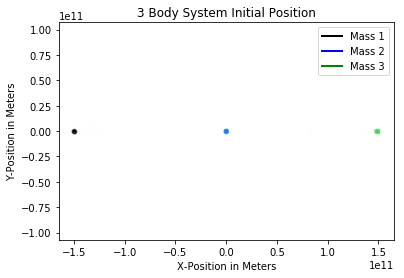
\includegraphics[width=1.0\linewidth]{3BodyDynamics6.png}
\end{center}
\end{figure}
\begin{figure}
\begin{center}
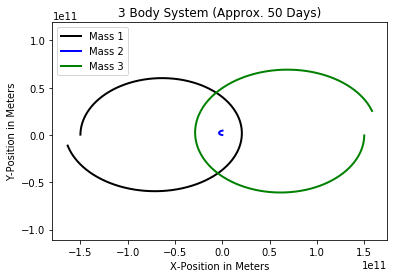
\includegraphics[width=1.0\linewidth]{3BodyDynamics9.png}
\end{center}
\end{figure}
\end{multicols}
\end{frame}
%------------------------------------------------
%	3-Body Motion (12)
%------------------------------------------------
\begin{frame}
\frametitle{3-Body Motion (12)}
The purpose behind these plots are to depict smaller stars orbiting once another and show the non-predictable behavior of these systems.
\begin{multicols}{2}
\begin{figure}
\begin{center}
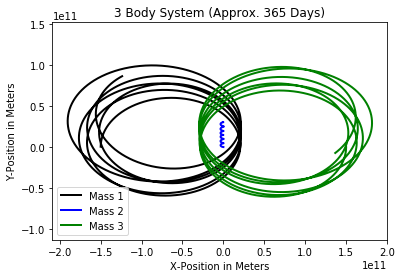
\includegraphics[width=1.0\linewidth]{3BodyDynamics10.png}
\end{center}
\end{figure}
\begin{figure}
\begin{center}
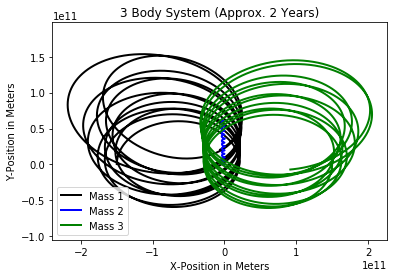
\includegraphics[width=1.0\linewidth]{3BodyDynamics11.png}
\end{center}
\end{figure}
\end{multicols}
\end{frame}
%------------------------------------------------
%	3-Body Motion (13)
%------------------------------------------------
\begin{frame}
\frametitle{3-Body Motion (13)}
And lastly, the final plot of this system can be seen below.
\begin{figure}
\begin{center}
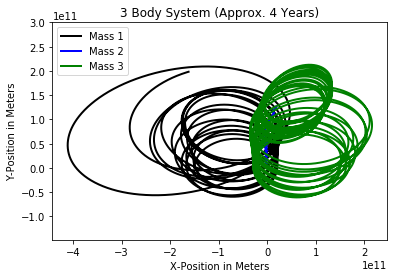
\includegraphics[width=0.90\linewidth]{3BodyDynamics12.png}
\end{center}
\end{figure}
\end{frame}
%------------------------------------------------
%	3-Body Motion (14)
%------------------------------------------------
\subsection{\tiny{Stability of 3-Body Motion}}
\begin{frame}
\frametitle{3-Body Motion (14)}
These plots show that certain systems are more unstable than others.\\
\vspace{20pt}
Larger mass ratios yield more stable ternary star systems.\\
\vspace{20pt}
Masses that are very similar in a system tend to yield more unstable systems that eventually devolve into binary star systems.
\end{frame}
%------------------------------------------------
%	3-Body Motion (15)
%------------------------------------------------
\begin{frame}
\frametitle{3-Body Motion (15)}
The stability of these orbits comes into question, how can we determine if an orbit is going to be stable?
\begin{equation}
\frac{a_{out}}{a_{in}}|_{crit}=\frac{2.8}{1-e_{out}}\Big(1-\frac{0.3i}{\pi}\Big)\cdot\Big(\frac{(1.0+q_{out})\cdot(1+e_{out})}{\sqrt{1-e_{out}}}\Big)^{2/5}
\end{equation}
Orbits are considered unstable if $\frac{a_{out}}{a_{in}}<\frac{a_{out}}{a_{in}}|_{crit}$ where $i=\pi/2$ and 
$q_{out}=\frac{m_3}{m_1+m_2}$ \cite{Triple Star}. $a_{out}$ and $a_{in}$ are the outer and inner semi major axis' of these orbits.\\
\vspace{20pt}
Stability of these orbits are largely determined on the eccentricity of the outer star in ternary star orbits.
\end{frame}
%------------------------------------------------
%	3-Body Motion (16)
%------------------------------------------------
\begin{frame}
\frametitle{3-Body Motion (16)}
Here is an example of real three body orbit.
\begin{multicols}{2}
\begin{figure}
\begin{center}
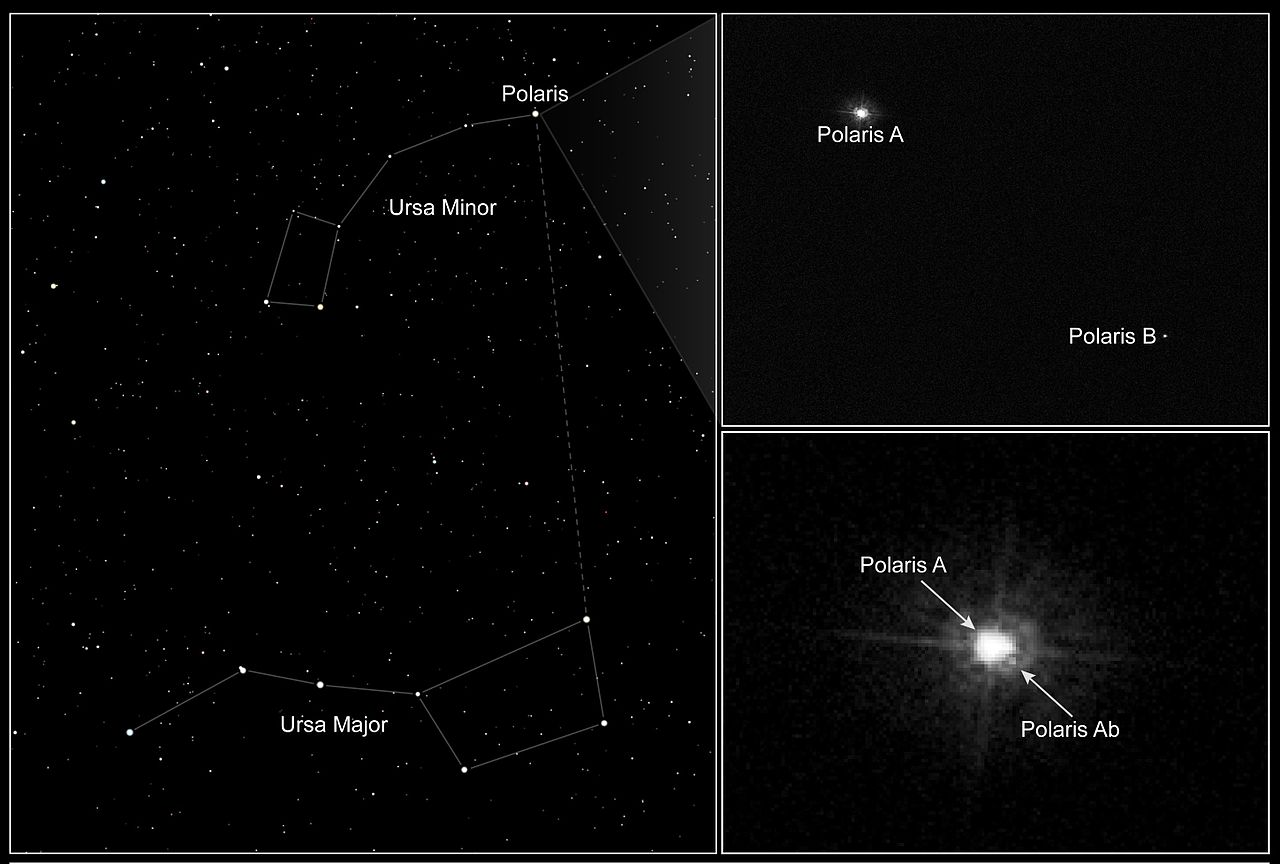
\includegraphics[width=1.0\linewidth]{PolarisA.jpg}
\end{center}
\end{figure}
\begin{figure}
\begin{center}
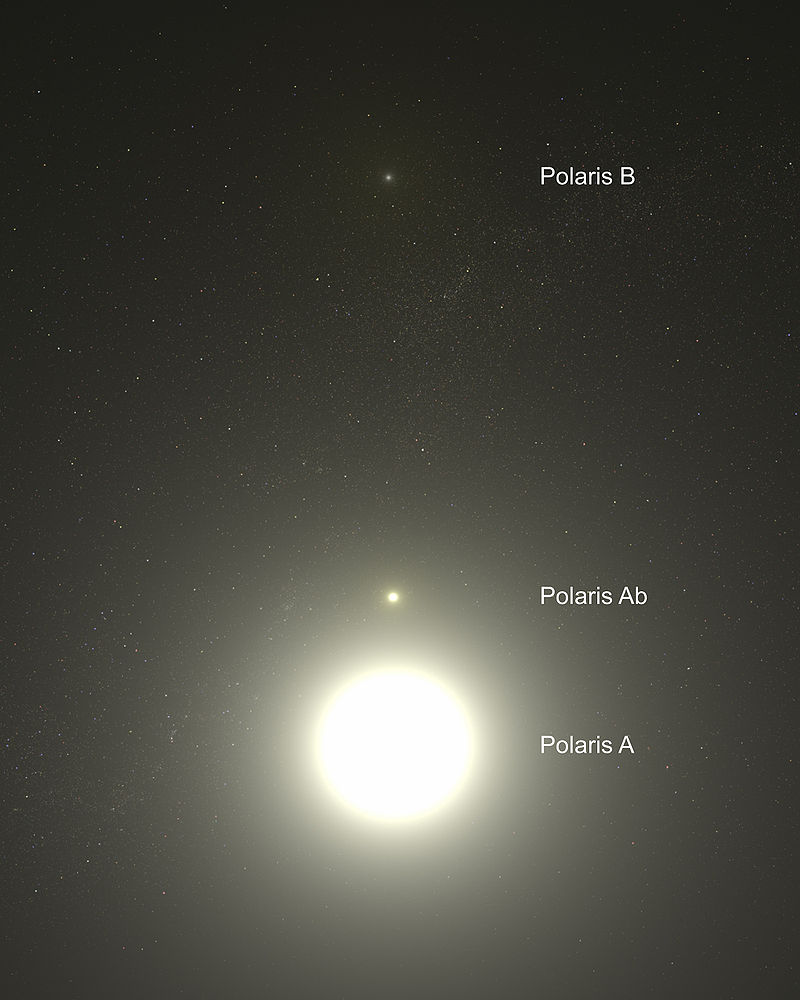
\includegraphics[width=1.0\linewidth]{PolarisB.jpg}
\end{center}
\end{figure}
\end{multicols}
\end{frame}
%------------------------------------------------
%	Conclusions
%------------------------------------------------
\section{Conclusions}
\begin{frame}
\frametitle{Conclusions}
The three body systems are chaotic and usually have unpredictable orbits unless they are under ideal initial conditions. \\
\vspace{10pt}
There are an infinite amount of solutions for the three body system. Each solution arises from the initial conditions and thus is why we require numerical solutions. \\
\vspace{10pt}
In the search of stable ternary star systems we should be looking for large mass ratios and not very elliptic orbits.
\end{frame}
%------------------------------------------------
%	References
%------------------------------------------------
\begin{frame}
\frametitle{References}
\footnotesize{
\begin{thebibliography}{99}
\bibitem{Byrd}
\tiny{Byrd, D. (2017, October 27). Perseus the Hero and a Demon Star. Retrieved September 29, 2019, from \url{https://earthsky.org/tonight/close-up-on-constellation-perseus-the-hero.}}
\bibitem{Cartoon Throwing Ball}
\tiny{(n.d.). How to Animate a Character Throwing a Ball. Retrieved from \url{https://design.tutsplus.com/tutorials/how-to-animate-a-character-throwing-a-ball--cms-26207}}
\bibitem{CSIRO}
\tiny{CSIRO Australia Telescope National Facility, \& Epping NSW. (2019, May 8). Introduction to Binary Stars. Retrieved September 29, 2019, from \url{https://www.atnf.csiro.au/outreach/education/senior/astrophysics/binary_intro.html}}
\bibitem{Forward Euler Difference Scheme}
\tiny{(n.d.). Euler Forward Method. Retrieved from \url{http://mathworld.wolfram.com/EulerForwardMethod.html}}
\bibitem{Perseus}
\tiny{Perseus Constellation - Facts About Perseus. (n.d.). Retrieved from \url{https://www.solarsystemquick.com/universe/perseus-constellation.htm.}}
\bibitem{Polaris}
\tiny{Polaris. (2019, October 18). Retrieved from \url{https://en.wikipedia.org/wiki/Polaris.}}
\bibitem{Triple Star}
\tiny{Toonen, S., \& Zwart1, S. P. (2016, December 23). The evolution of hierarchical triple star-systems. Retrieved from \url{https://comp-astrophys-cosmol.springeropen.com/articles/10.1186/s40668-016-0019-0.}}
\end{thebibliography}
}
\end{frame}
%------------------------------------------------
%	Questions
%------------------------------------------------
\begin{frame}
\frametitle{Questions?}
Any Questions?
\end{frame}
\end{document}
%----------------------------------------------------------------------------------------
%	Comment Headers
%----------------------------------------------------------------------------------------

%----------------------------------------------------------------------------------------

%------------------------------------------------

%----------------------------------------------------------------------------------------
%	
%----------------------------------------------------------------------------------------

%------------------------------------------------
%	
%------------------------------------------------
